\documentclass[tikz,border=5pt]{standalone}
\usepackage{tikz}
\usepackage{graphicx}
\pagestyle{empty}
\begin{document}
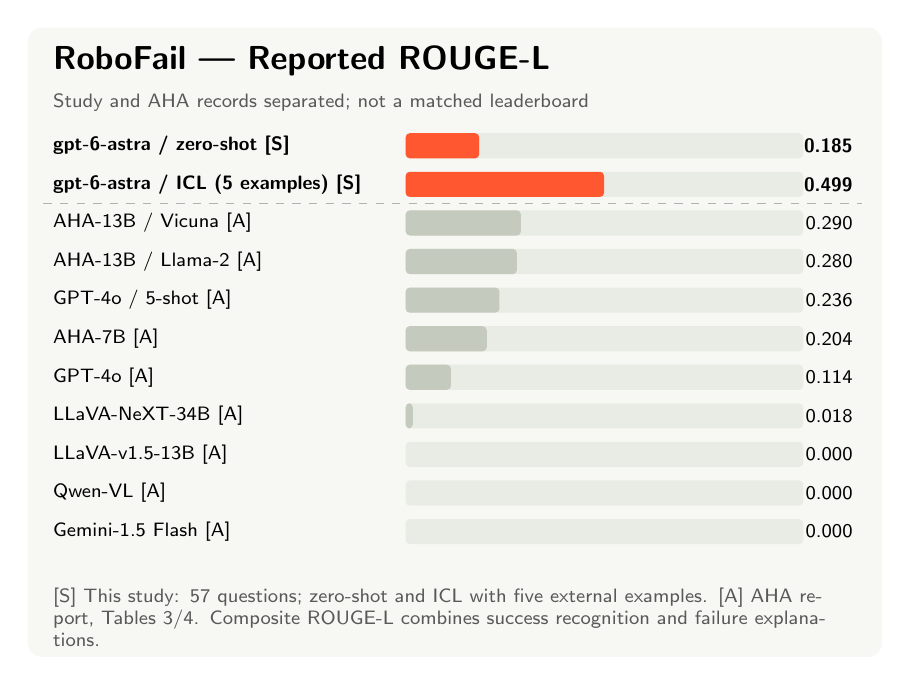
\begin{tikzpicture}[x=1cm,y=1cm,font=\sffamily]
\definecolor{rfbg}{HTML}{F7F8F3}
\definecolor{rftrack}{HTML}{E9ECE4}
\definecolor{rfgray}{HTML}{C5CABF}
\definecolor{rforange}{HTML}{FF572F}
\fill[rfbg,rounded corners=5pt] (-.2,1.2) rectangle (10.65,-6.789999999999999);
\node[anchor=west,font=\sffamily\bfseries\large] at (0,.77) {RoboFail | Reported ROUGE-L};
\node[anchor=west,font=\sffamily\scriptsize,text=black!65] at (0,.25) {Study and AHA records separated; not a matched leaderboard};
\node[anchor=west,font=\sffamily\scriptsize\bfseries] at (0,-0.3) {gpt-6-astra / zero-shot [S]};
\fill[rftrack,rounded corners=1.5pt] (4.6,-0.45999999999999996) rectangle (9.65,-0.13999999999999999);
\fill[rforange,rounded corners=1.5pt] (4.6,-0.45999999999999996) rectangle (5.534249999999999,-0.13999999999999999);
\node[anchor=east,font=\sffamily\scriptsize\bfseries] at (10.4,-0.3) {0.185};
\node[anchor=west,font=\sffamily\scriptsize\bfseries] at (0,-0.79) {gpt-6-astra / ICL (5 examples) [S]};
\fill[rftrack,rounded corners=1.5pt] (4.6,-0.9500000000000001) rectangle (9.65,-0.63);
\fill[rforange,rounded corners=1.5pt] (4.6,-0.9500000000000001) rectangle (7.119949999999999,-0.63);
\node[anchor=east,font=\sffamily\scriptsize\bfseries] at (10.4,-0.79) {0.499};
\draw[dashed,black!30] (0,-1.03) -- (10.4,-1.03);
\node[anchor=west,font=\sffamily\scriptsize] at (0,-1.28) {AHA-13B / Vicuna [A]};
\fill[rftrack,rounded corners=1.5pt] (4.6,-1.44) rectangle (9.65,-1.12);
\fill[rfgray,rounded corners=1.5pt] (4.6,-1.44) rectangle (6.0645,-1.12);
\node[anchor=east,font=\sffamily\scriptsize] at (10.4,-1.28) {0.290};
\node[anchor=west,font=\sffamily\scriptsize] at (0,-1.77) {AHA-13B / Llama-2 [A]};
\fill[rftrack,rounded corners=1.5pt] (4.6,-1.93) rectangle (9.65,-1.61);
\fill[rfgray,rounded corners=1.5pt] (4.6,-1.93) rectangle (6.013999999999999,-1.61);
\node[anchor=east,font=\sffamily\scriptsize] at (10.4,-1.77) {0.280};
\node[anchor=west,font=\sffamily\scriptsize] at (0,-2.26) {GPT-4o / 5-shot [A]};
\fill[rftrack,rounded corners=1.5pt] (4.6,-2.42) rectangle (9.65,-2.0999999999999996);
\fill[rfgray,rounded corners=1.5pt] (4.6,-2.42) rectangle (5.791799999999999,-2.0999999999999996);
\node[anchor=east,font=\sffamily\scriptsize] at (10.4,-2.26) {0.236};
\node[anchor=west,font=\sffamily\scriptsize] at (0,-2.75) {AHA-7B [A]};
\fill[rftrack,rounded corners=1.5pt] (4.6,-2.91) rectangle (9.65,-2.59);
\fill[rfgray,rounded corners=1.5pt] (4.6,-2.91) rectangle (5.630199999999999,-2.59);
\node[anchor=east,font=\sffamily\scriptsize] at (10.4,-2.75) {0.204};
\node[anchor=west,font=\sffamily\scriptsize] at (0,-3.2399999999999998) {GPT-4o [A]};
\fill[rftrack,rounded corners=1.5pt] (4.6,-3.4) rectangle (9.65,-3.0799999999999996);
\fill[rfgray,rounded corners=1.5pt] (4.6,-3.4) rectangle (5.1757,-3.0799999999999996);
\node[anchor=east,font=\sffamily\scriptsize] at (10.4,-3.2399999999999998) {0.114};
\node[anchor=west,font=\sffamily\scriptsize] at (0,-3.7299999999999995) {LLaVA-NeXT-34B [A]};
\fill[rftrack,rounded corners=1.5pt] (4.6,-3.8899999999999997) rectangle (9.65,-3.5699999999999994);
\fill[rfgray,rounded corners=1.5pt] (4.6,-3.8899999999999997) rectangle (4.6909,-3.5699999999999994);
\node[anchor=east,font=\sffamily\scriptsize] at (10.4,-3.7299999999999995) {0.018};
\node[anchor=west,font=\sffamily\scriptsize] at (0,-4.22) {LLaVA-v1.5-13B [A]};
\fill[rftrack,rounded corners=1.5pt] (4.6,-4.38) rectangle (9.65,-4.06);
\node[anchor=east,font=\sffamily\scriptsize] at (10.4,-4.22) {0.000};
\node[anchor=west,font=\sffamily\scriptsize] at (0,-4.71) {Qwen-VL [A]};
\fill[rftrack,rounded corners=1.5pt] (4.6,-4.87) rectangle (9.65,-4.55);
\node[anchor=east,font=\sffamily\scriptsize] at (10.4,-4.71) {0.000};
\node[anchor=west,font=\sffamily\scriptsize] at (0,-5.2) {Gemini-1.5 Flash [A]};
\fill[rftrack,rounded corners=1.5pt] (4.6,-5.36) rectangle (9.65,-5.04);
\node[anchor=east,font=\sffamily\scriptsize] at (10.4,-5.2) {0.000};
\node[anchor=north west,text width=10cm,font=\sffamily\scriptsize,text=black!65] at (0,-5.79) {[S] This study: 57 questions; zero-shot and ICL with five external examples. [A] AHA report, Tables 3/4. Composite ROUGE-L combines success recognition and failure explanations.};
\end{tikzpicture}

\end{document}
